
% This LaTeX was auto-generated from an M-file by MATLAB.
% To make changes, update the M-file and republish this document.

\documentclass{article}
\usepackage{graphicx}
\usepackage{color}

\sloppy
\definecolor{lightgray}{gray}{0.5}
\setlength{\parindent}{10pt}
\usepackage[margin=1in]{geometry}

\begin{document}

\title{Dynamical Adaptation in ORNs}
\author{Srinivas Gorur-Shandilya}
\maketitle

    
    
\section*{Fitting the Dynamical Adaptation Model to ORN Responses}

\begin{par}
In this document, I will try to fit the Dynamical Adaptation (DA) model to data from random stimulation experiments on ORNs. First, the DA model is fit to synthetic data generated by the DA model, and then is fit to real data. I then go through the analysis of the instantaneous gain for a linear model and the DA model, and characterize the fast adaptation properties of ORNs to this odour.
\end{par} \vspace{1em}

\subsection*{Contents}

\begin{itemize}
\setlength{\itemsep}{-1ex}
   \item Synthetic Data: Fitting the DA model
   \item Synthetic Data: Gain Analysis
   \item Fitting DA Model to real data
   \item Real Data: Gain Analysis
\end{itemize}


\subsection*{Synthetic Data: Fitting the DA model}

\begin{par}
The Dynamical Adaptation model has 8 parameters that need to be constrained. Setting one of them, $\tau_{r}$, to zero eliminates the need to solve a differential equation, and the response is given in closed form as a function of the stimulus. This greatly speeds up code execution.
\end{par} \vspace{1em}

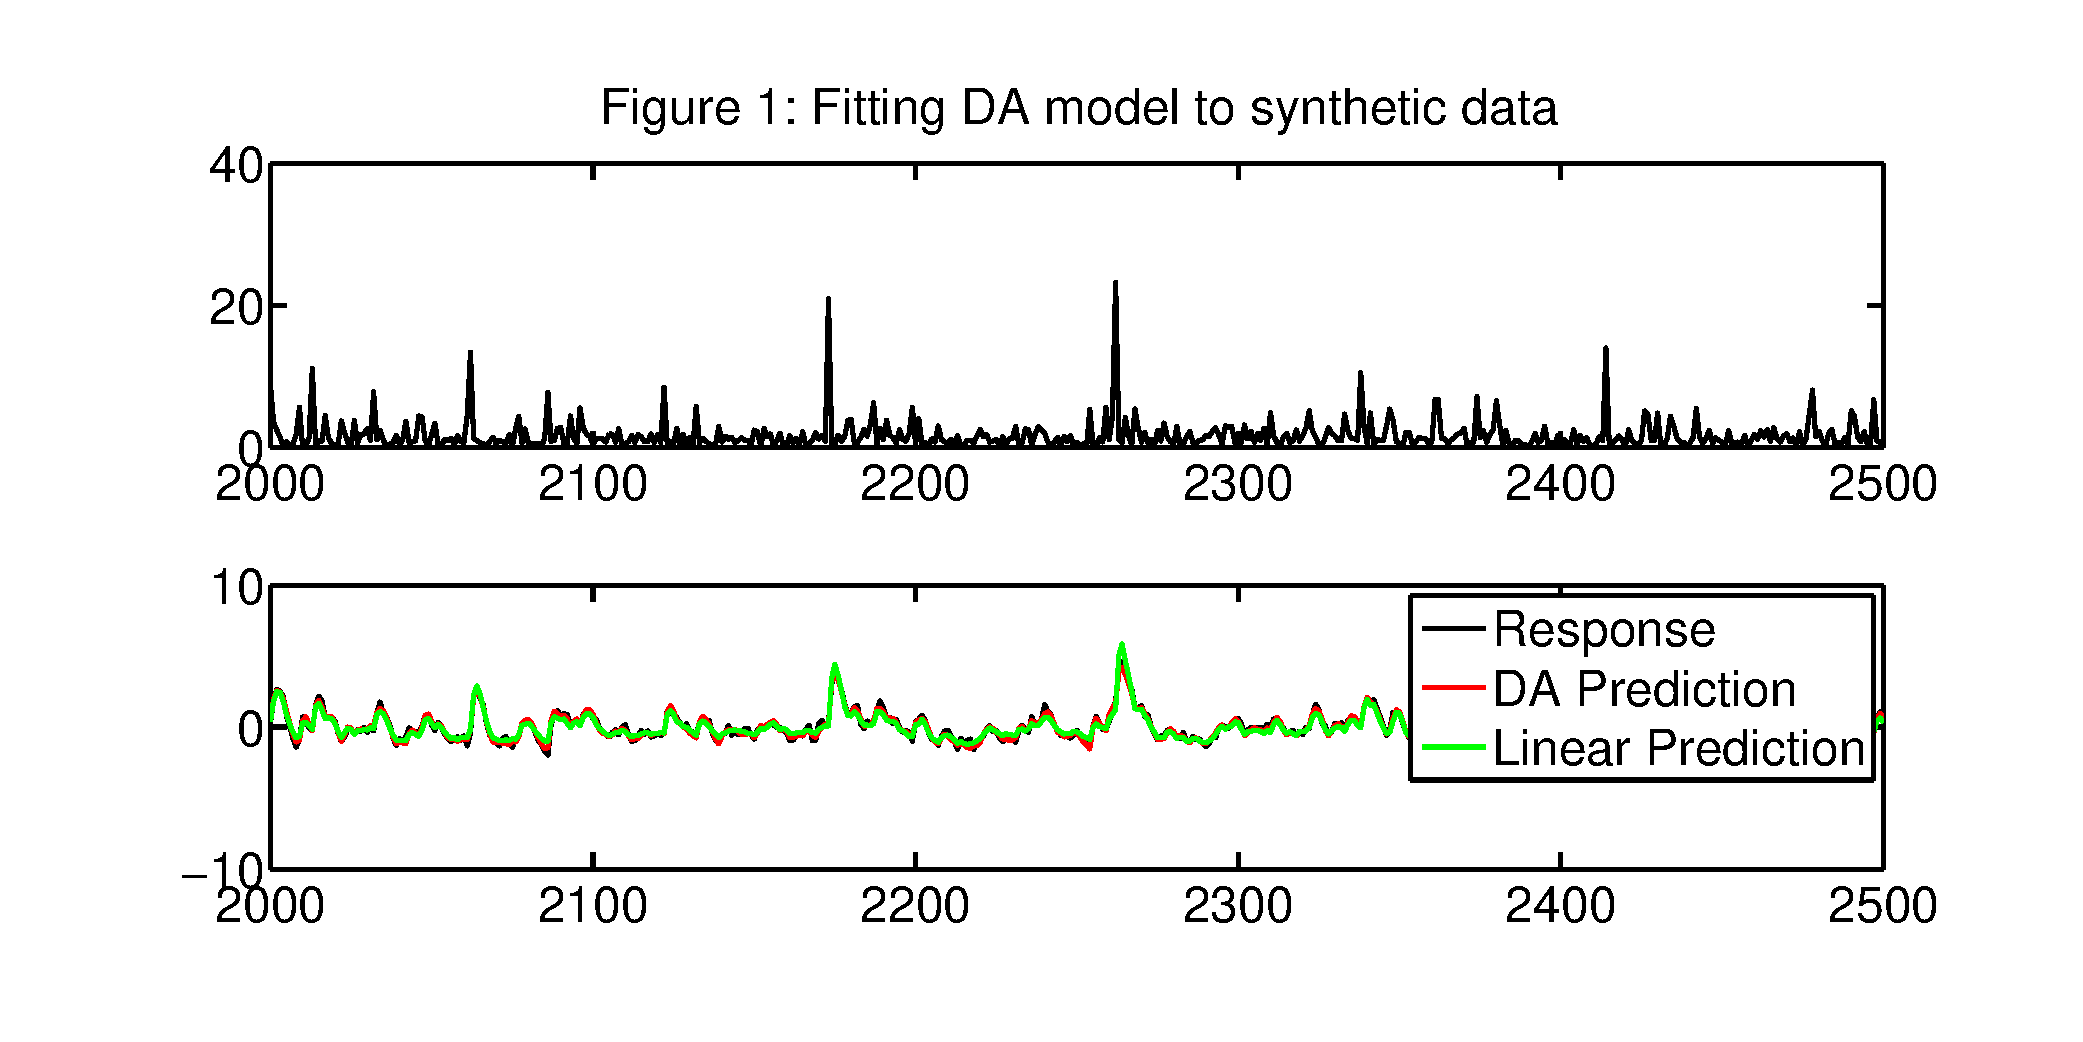
\includegraphics [width=\textwidth]{FittingDAModel_01.pdf}
\begin{par}
First, I will fit these 7 parameters to synthetic data, generated by running the DA model on exponentiated and filtered gaussian random noise input. In Figure 1, the top panel shows the input to the model. The bottom panel shows the model output (black), the linear prediction (green), and finally the DA model prediction (red).
\end{par} \vspace{1em}
\begin{par}
The DA model fits the data really well; the black line of the synthetic data is completely hidden by the red line of the DA model prediction. To fit the DA model, I used a genetic algorithm to perform a nearly-global search with integer constraints on $n_{y}$ and $n_{z}$, and $\gamma$ constrained to $[0,1]$
\end{par} \vspace{1em}
\begin{par}
The DA model seems to do a pretty good job estimating the data output. Is it better than the simple linear prediction? Here, we compare the r-square and the l-2 norm between the data and the fit. For the simple linear model, the r-square is
\end{par} \vspace{1em}

        \color{lightgray} \begin{verbatim}    0.8525

\end{verbatim} \color{black}
    \begin{par}
cf. the DA model fit, the rsquare is
\end{par} \vspace{1em}

        \color{lightgray} \begin{verbatim}    0.9613

\end{verbatim} \color{black}
    \begin{par}
The l-2 norm of the linear fit is
\end{par} \vspace{1em}

        \color{lightgray} \begin{verbatim}   36.9895

\end{verbatim} \color{black}
    \begin{par}
cf. l-2 norm of the DA fit is
\end{par} \vspace{1em}

        \color{lightgray} \begin{verbatim}   18.9649

\end{verbatim} \color{black}
    \begin{par}
The DA model fits the data much better, which makes sense as the stimulus is non-gaussian, and we have crafted the synthetic data set so that the DA model does the best job explaining its variance.
\end{par} \vspace{1em}


\subsection*{Synthetic Data: Gain Analysis}

\begin{par}
Sensors can exhibit fast adaptation to the stimulus, on a time-scale not dissimilar to the time-scale of response to the stimulus. In this analysis, we smooth the stimulus to the sensor over some arbitrary history window, and plot the actual response of the sensor to the model prediction for the top 10\% of smoothed stimulus input, and for the bottom 10\% of the smoothed stimulus input.
\end{par} \vspace{1em}
\begin{par}
In the figure below, we characterise the "fast adaptation" properties in the synthetic data.  The plot on the left compares the data (on the Y-axis) to the linear fit, while the plot on the right compares the data to the DA model fit. Several interesting features are visible:
\end{par} \vspace{1em}
\begin{enumerate}
\setlength{\itemsep}{-1ex}
   \item The best-fit lines to the top 10\% (red) and bottom 10\% (red) of stimulus have different slopes in the linear fit. In particular, the response to the stronger stimuli (red) has lower gain (smaller slope) than the response to the lower stimuli (green).
   \item This is not true for the fit to the DA model. The DA model does not systematically wrongly estimate the gain of the synthetic data, unlike the linear fit.
\end{enumerate}

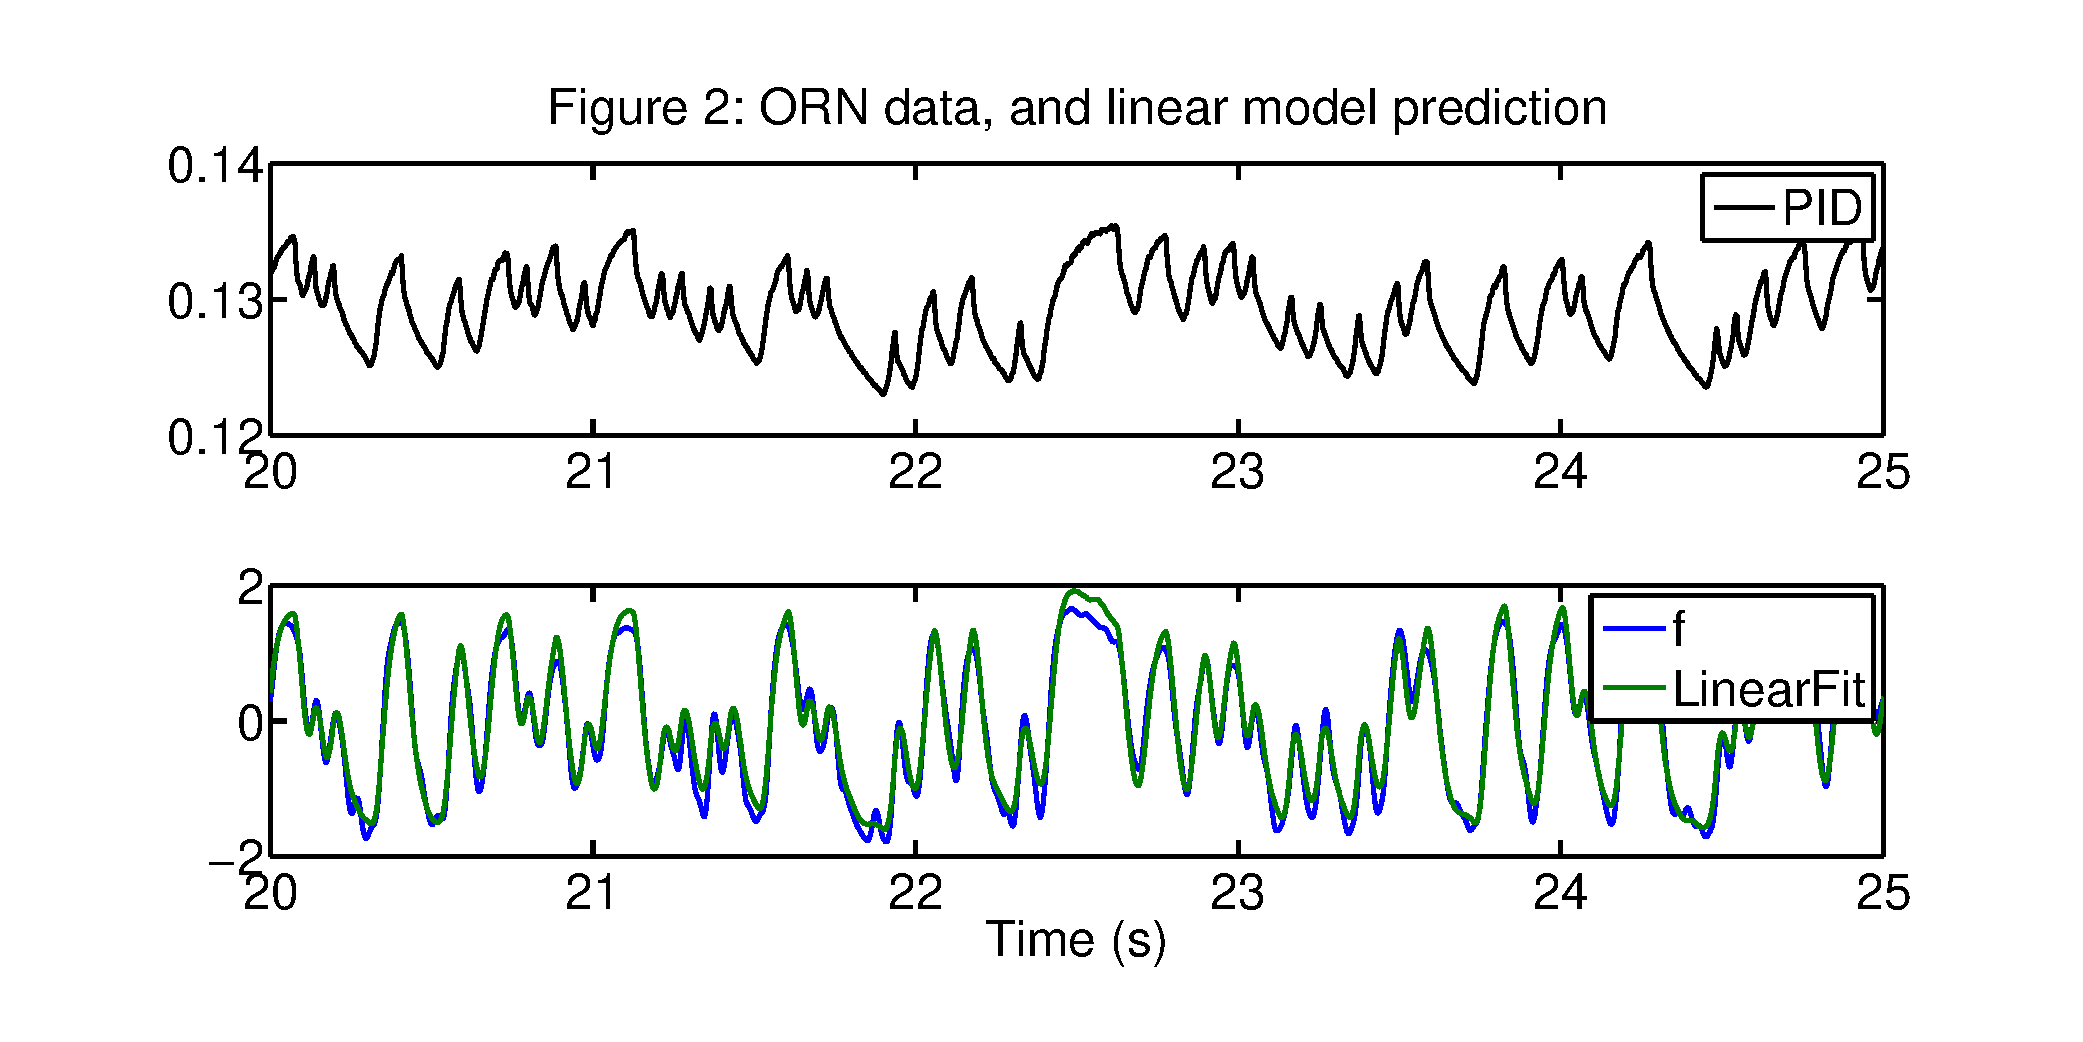
\includegraphics [width=\textwidth]{FittingDAModel_02.pdf}
\begin{par}
How does this vary with the length of the history window?  In the analysis above, we have kept the "window history" length fixed. How does varying this window change the separation of slopes of best fit lines for the top 10\% and the bottom 10\%?
\end{par} \vspace{1em}

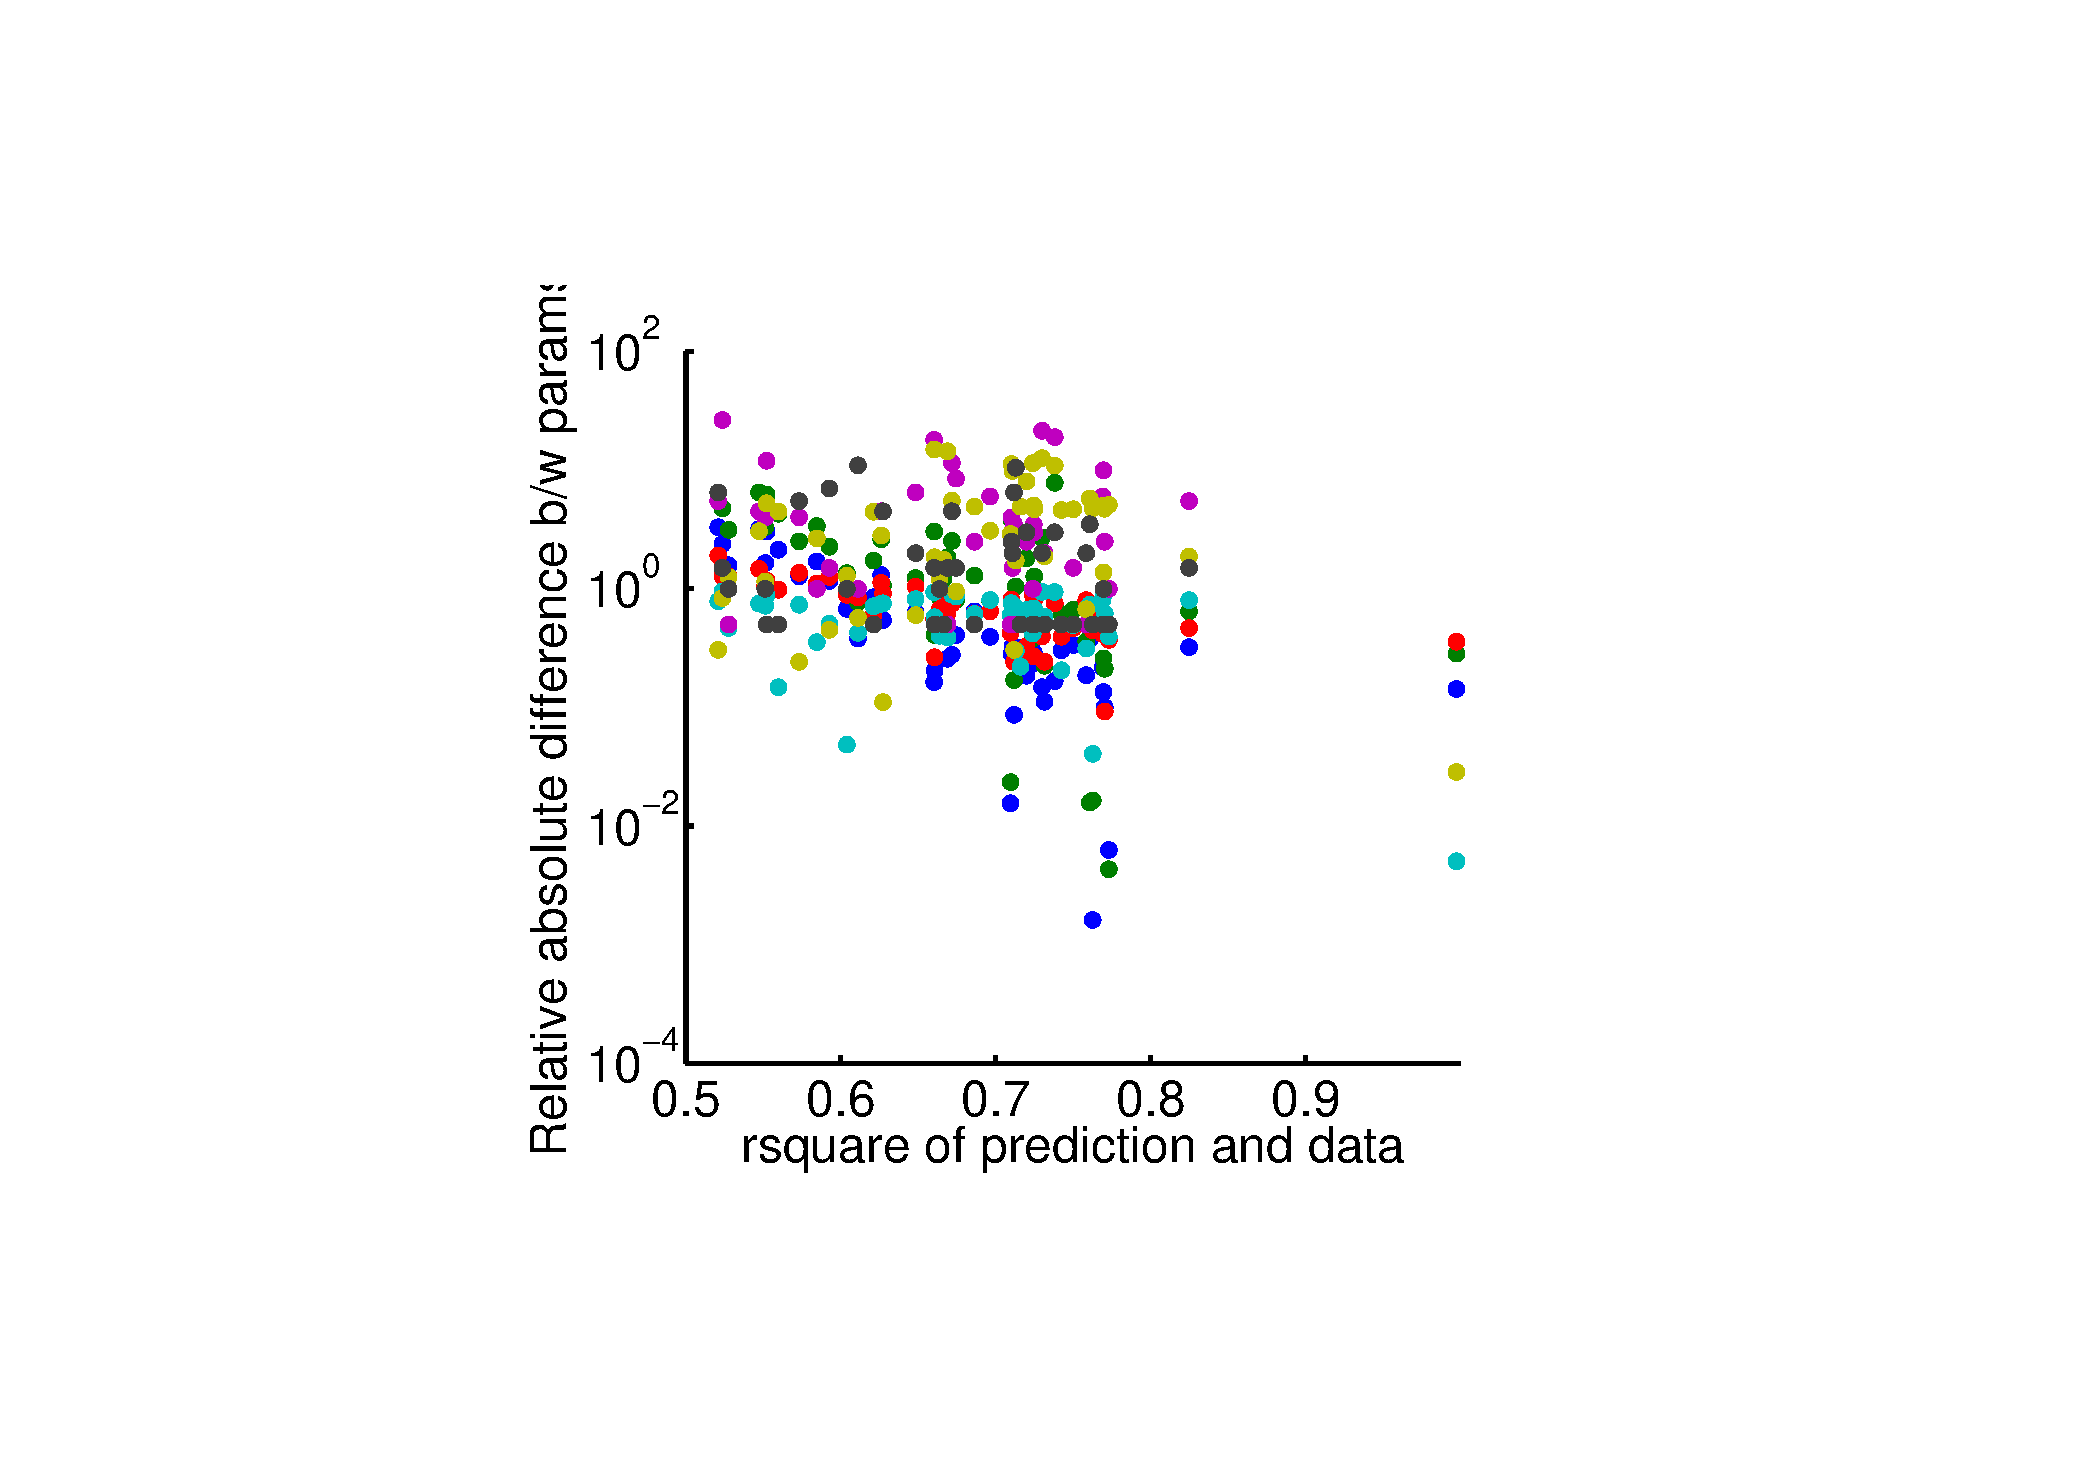
\includegraphics [width=\textwidth]{FittingDAModel_03.pdf}


\subsection*{Fitting DA Model to real data}

\begin{par}
Now that we know that we can fit the model, and that our optimisation algorithm works, we will try to fit real data. The following figure shows the sample data we use. The top panel shows the stimulus as measured by the PID, and the bottom panel shows the firing rate of the ORN. The firing rate has been divided by its standard deviation and has been mean subtracted. Also shown is the linear prediction of the firing rates.
\end{par} \vspace{1em}

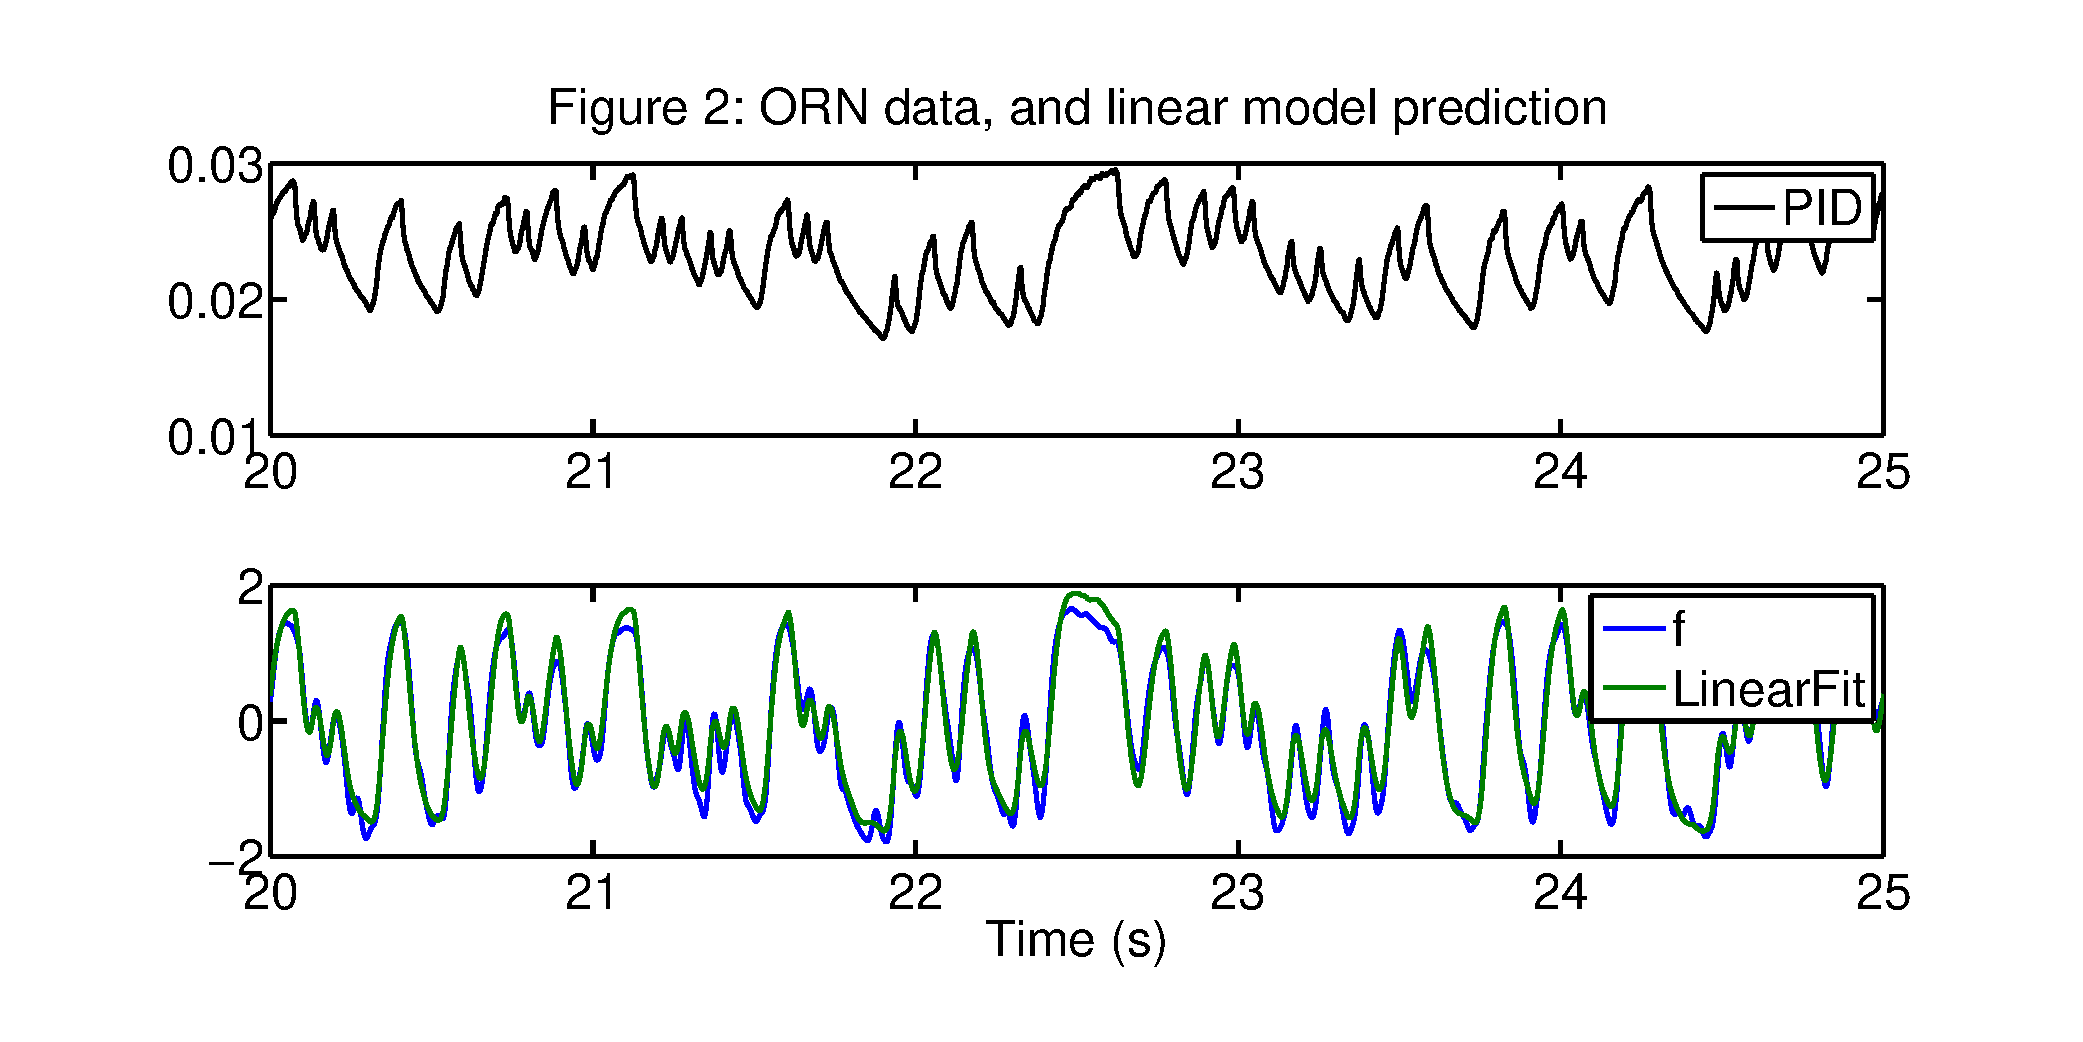
\includegraphics [width=\textwidth]{FittingDAModel_04.pdf}
\begin{par}
Now, we fit the DA model to the data using a pattern search optimisation (the type of optimisation doesn't matter. Pattern search is faster and converges to local minima faster than GA). $\gamma$ is constrained to $[0,1]$
\end{par} \vspace{1em}

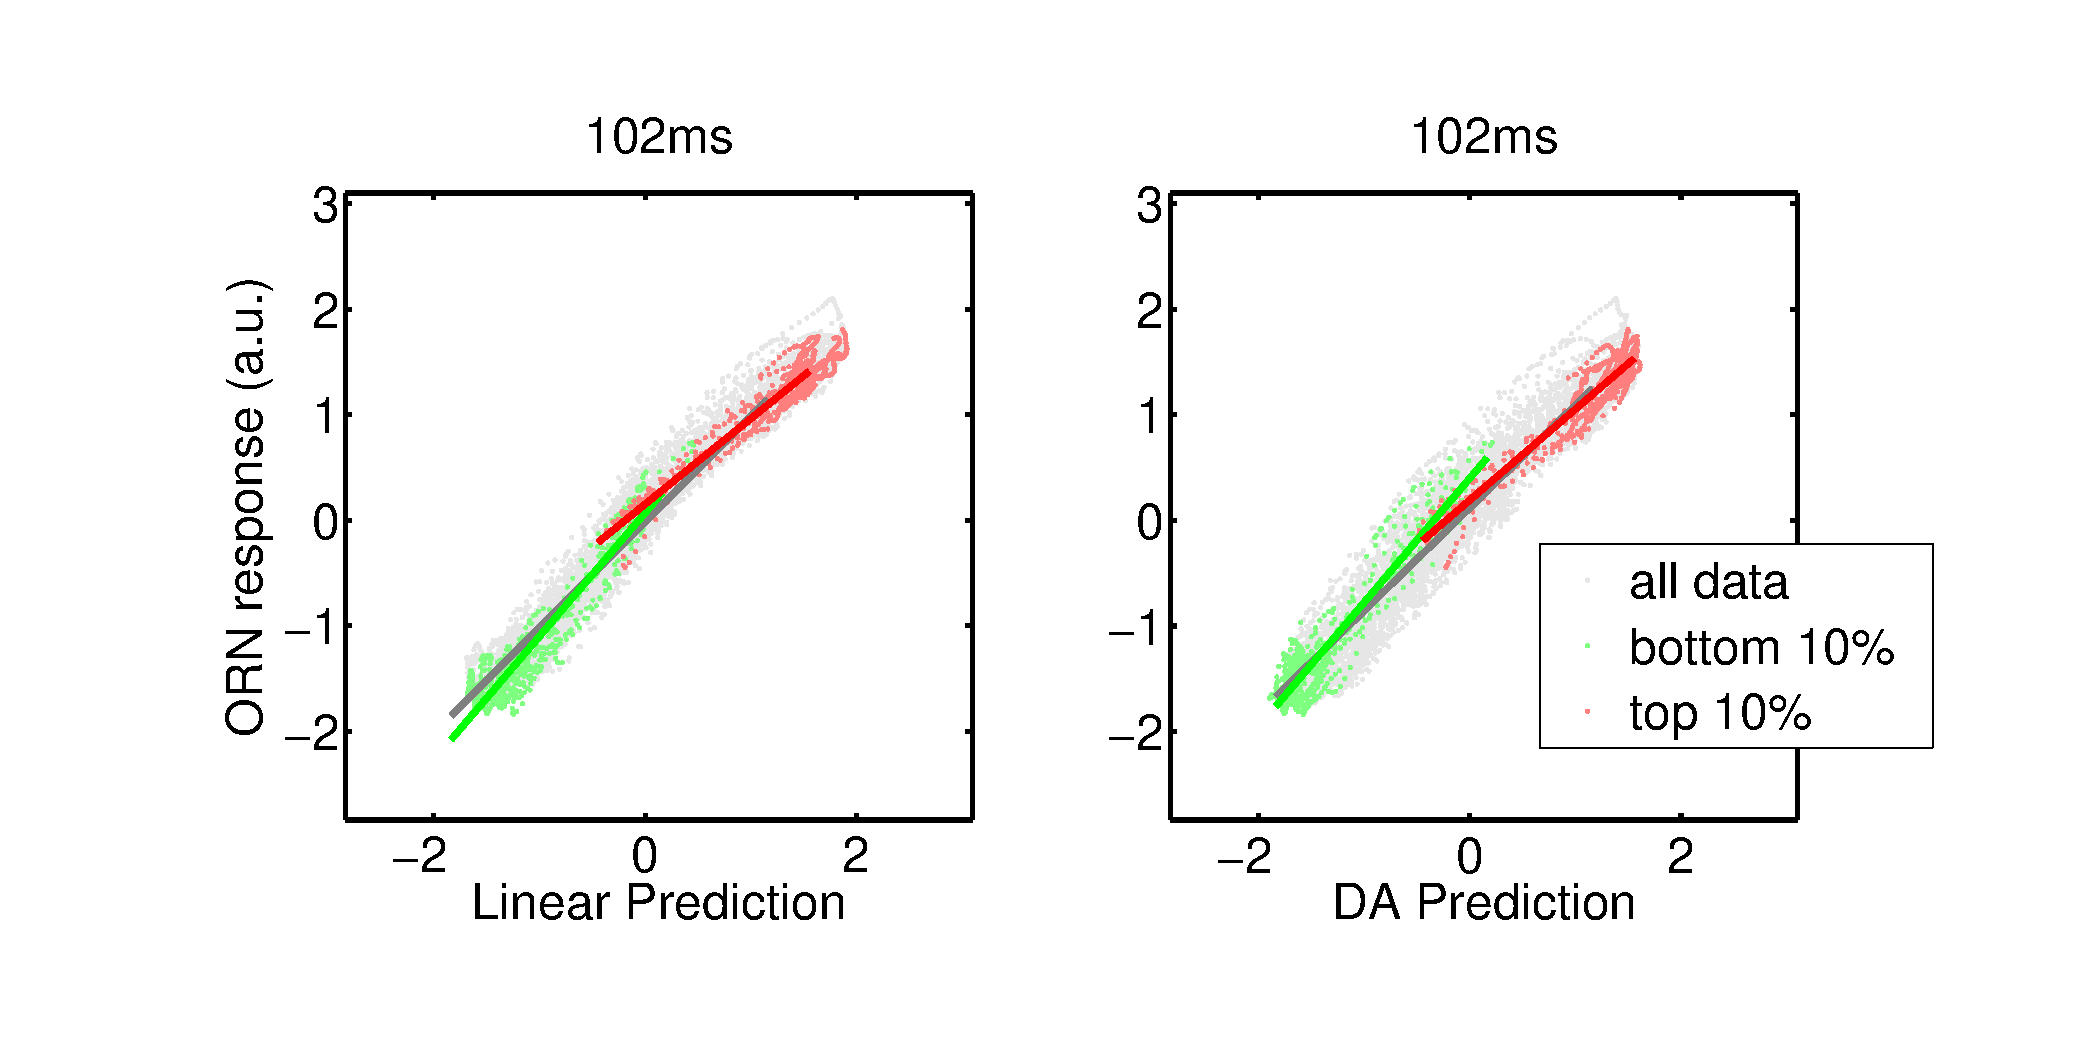
\includegraphics [width=\textwidth]{FittingDAModel_05.pdf}
\begin{par}
The DA model seems to do a pretty good job estimating the ORN output. Is it better than the simple linear prediction? Here, we compare the r-square and the l-2 norm between the data and the fit. For the simple linear model, the r-square is
\end{par} \vspace{1em}

        \color{lightgray} \begin{verbatim}    0.9506

\end{verbatim} \color{black}
    \begin{par}
cf. for the DA model fit, the rsquare is
\end{par} \vspace{1em}

        \color{lightgray} \begin{verbatim}    0.9432

\end{verbatim} \color{black}
    \begin{par}
The l-2 norm of the linear fit is
\end{par} \vspace{1em}

        \color{lightgray} \begin{verbatim}   17.4152

\end{verbatim} \color{black}
    \begin{par}
cf. l-2 norm of the DA fit is
\end{par} \vspace{1em}

        \color{lightgray} \begin{verbatim}   18.4932

\end{verbatim} \color{black}
    

\subsection*{Real Data: Gain Analysis}

\begin{par}
We can perform a similar gain analysis like we did on the synthetic data on the real data from the ORN. The plot on the left compares the ORN response data (on the Y-axis) to the linear fit, while the plot on the right compares the data to the DA model fit.
\end{par} \vspace{1em}

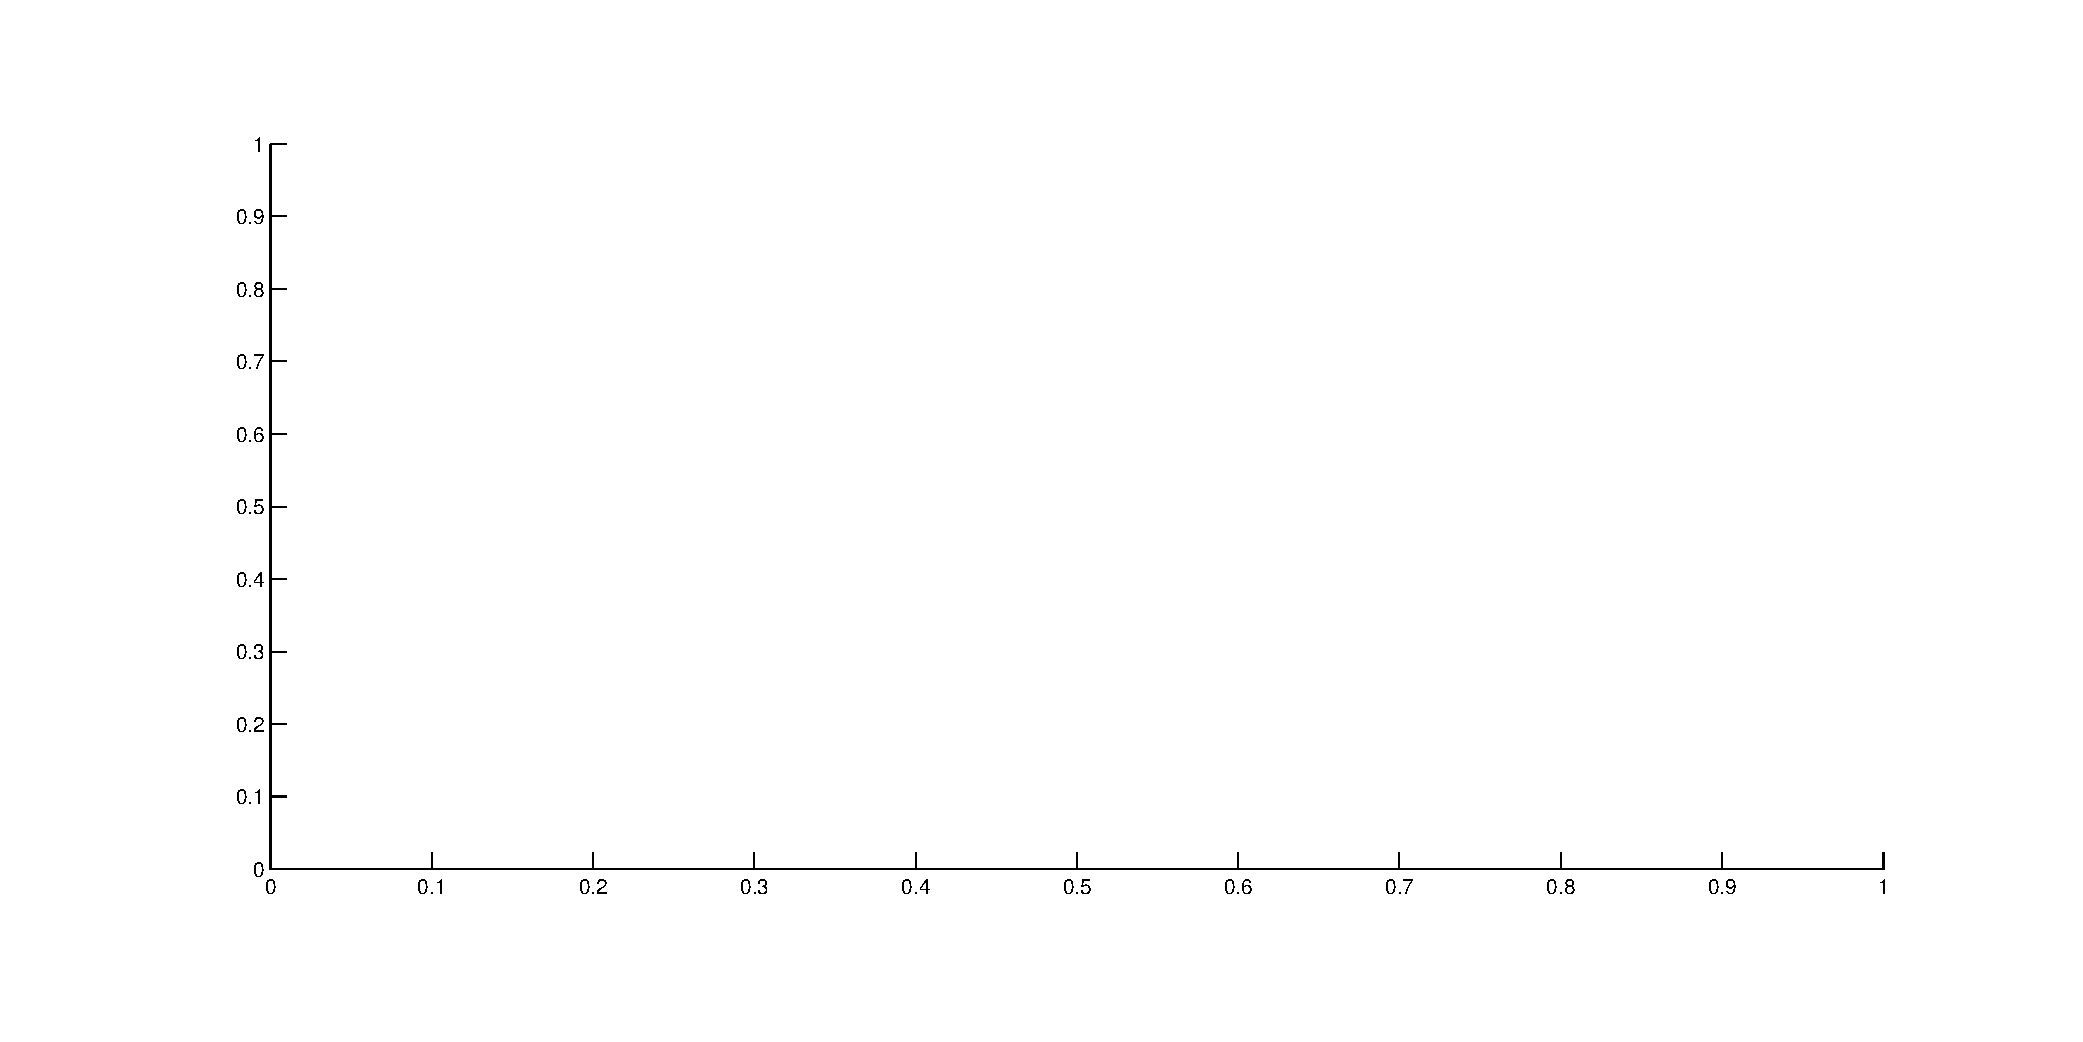
\includegraphics [width=\textwidth]{FittingDAModel_06.pdf}
\begin{par}
In the analysis above, we have kept the "window history" length fixed at \ensuremath{\tilde{\;}}100ms. How does varying this window change the separation of slopes of best fit lines for the top 10\% and the bottom 10\%?
\end{par} \vspace{1em}
\begin{par}
And we can do the same thing for the ORN response data.
\end{par} \vspace{1em}

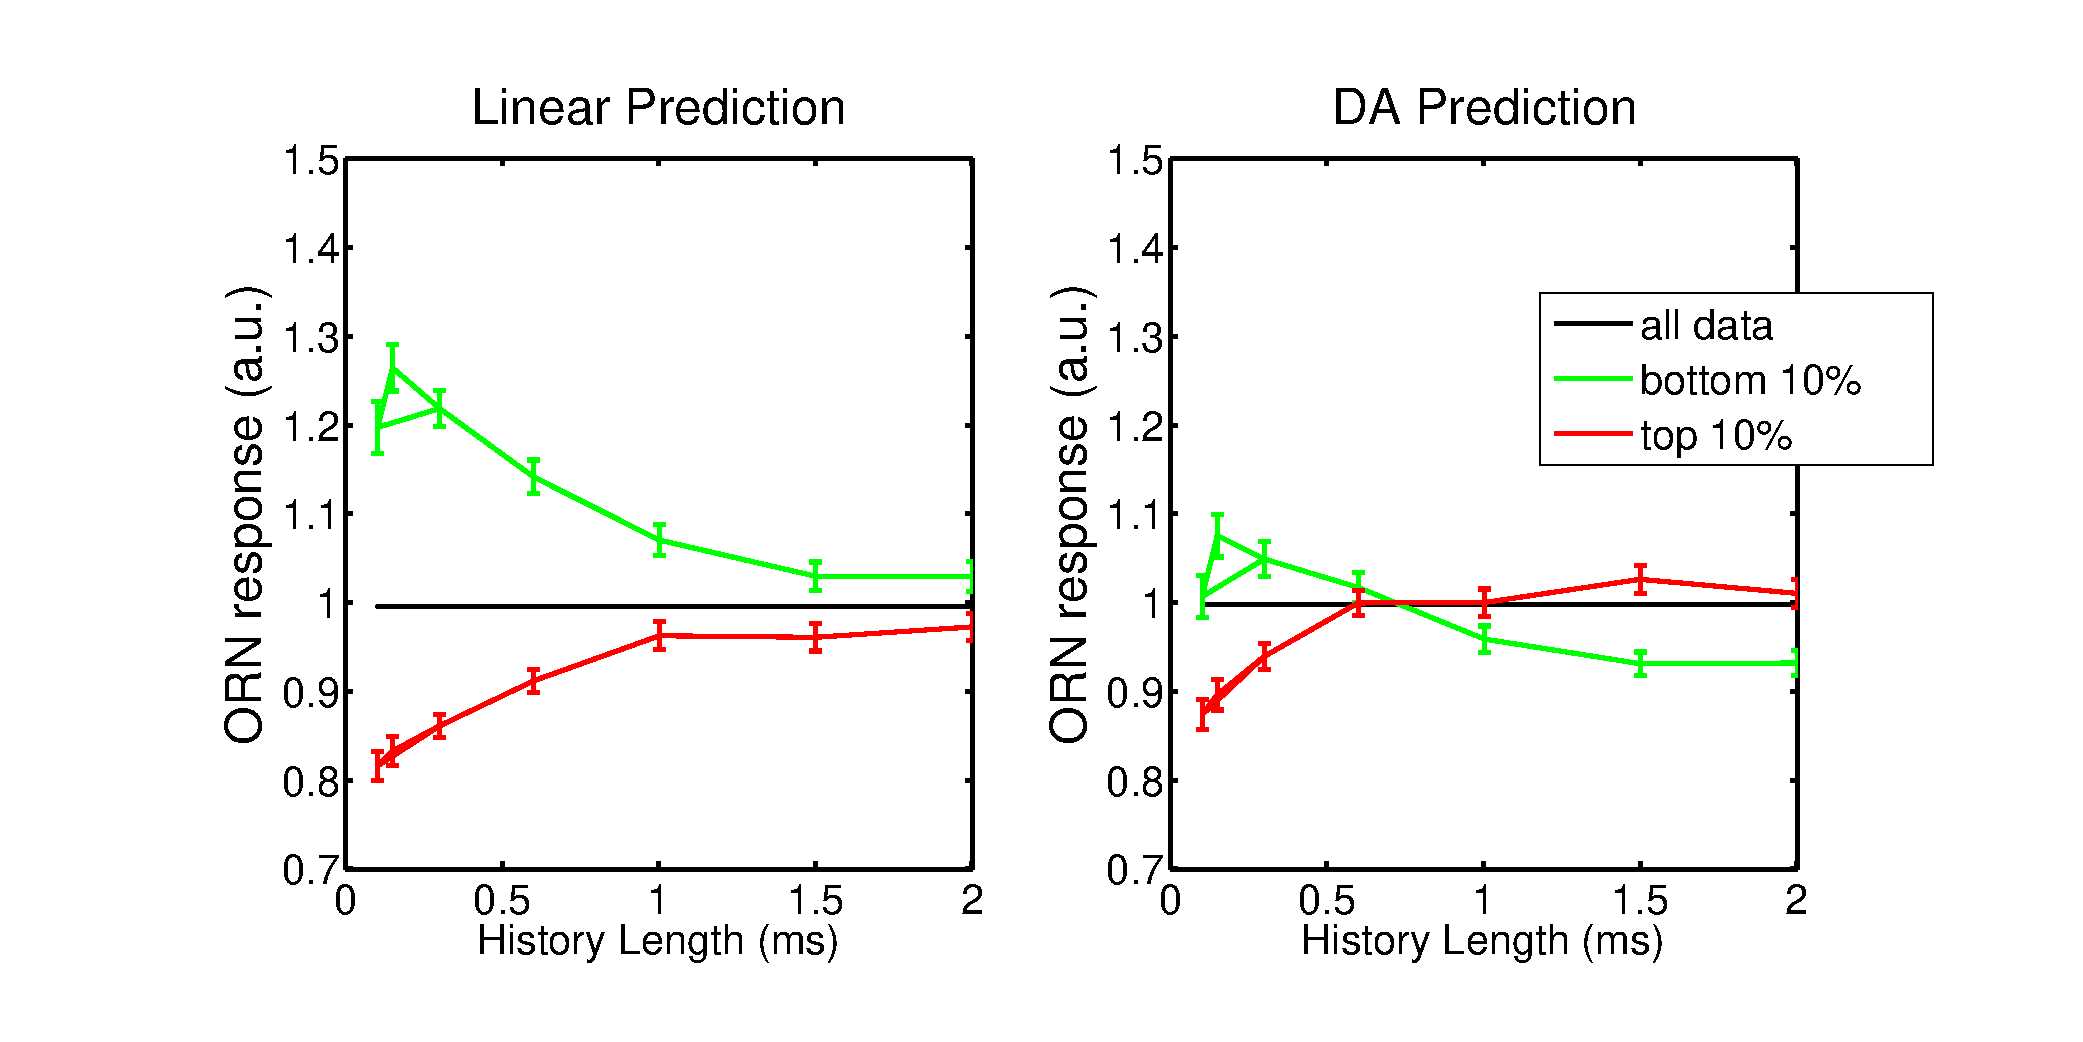
\includegraphics [width=\textwidth]{FittingDAModel_07.pdf}



\end{document}
    
